\documentclass[../main.tex]{subfiles} % NEW VERSION IS CASE.tex
\title{Foundations: A Blueprint for Æthernet}
\begin{document}

\section{A Blueprint for Æthernet Protocol}  
\begin{marginfigure}
  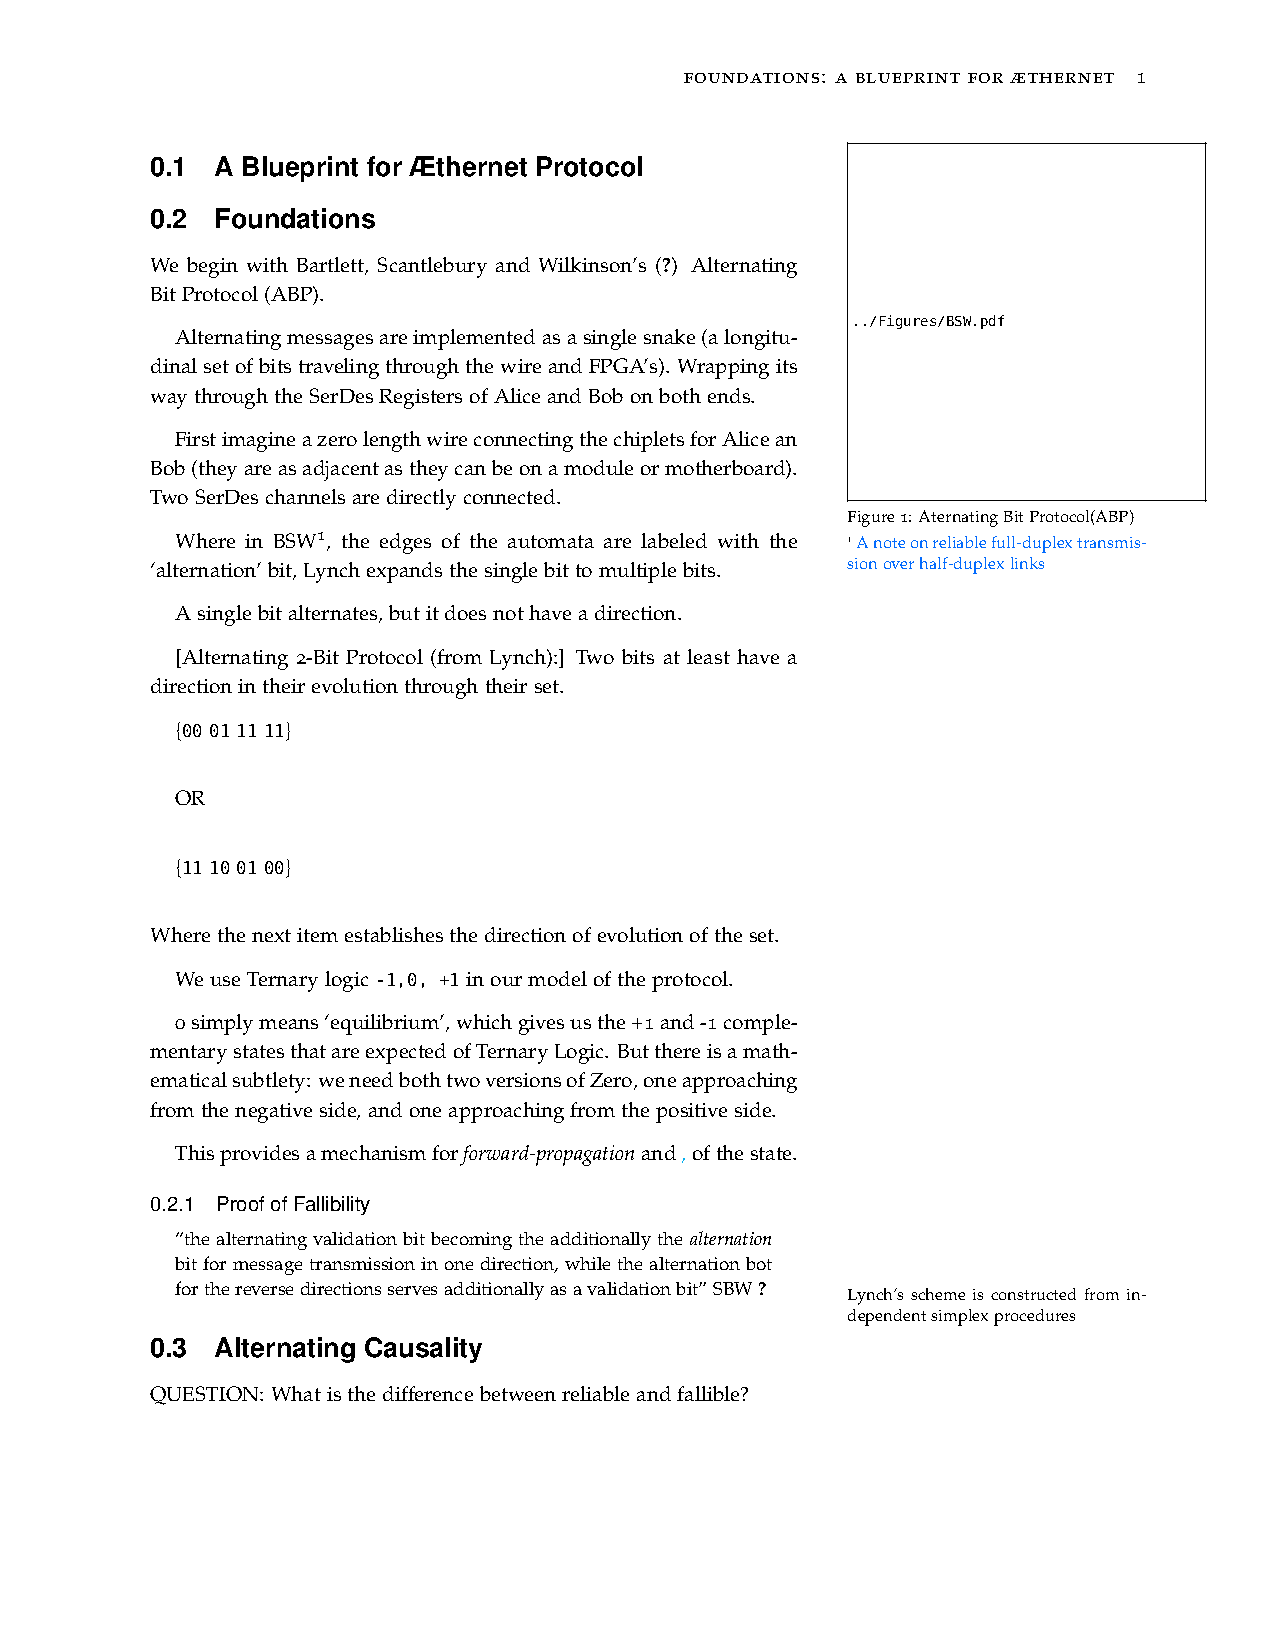
\includegraphics[width=1.2\linewidth]{../Figures/BSW.pdf}
  \caption{Aternating Bit Protocol(ABP)}
\end{marginfigure}

\section{Foundations}

We begin with Bartlett, Scantlebury and Wilkinson's  (\cite{BSW})  Alternating Bit Protocol (ABP).

Alternating messages are implemented as a single snake (a longitudinal set of bits traveling through the wire and FPGA's). Wrapping its way through the SerDes Registers of Alice and Bob on both ends.

First imagine a zero length wire connecting the chiplets for Alice an Bob (they are as adjacent as they can be on a module or motherboard). Two SerDes channels are directly connected. 

Where in BSW\sidenote{\href{https://dl.acm.org/doi/abs/10.1145/362946.362970}{A note on reliable full-duplex transmission over half-duplex links}}, the edges of the automata are labeled with the `alternation' bit, Lynch expands the single bit to multiple bits.

A single bit alternates, but it does not have a direction.

\begin{highlightbox}[Alternating 2-Bit Protocol (from Lynch):]
Two bits at least have a direction in their evolution through their set.
\end{highlightbox}

 
	 \{\texttt{00} {\texttt{01} {\texttt{11} {\texttt{11}\} 
	 
	 \bigskip
	 
	OR
	
	\bigskip
	
 	 \{\texttt{11} {\texttt{10} {\texttt{01} {\texttt{00}\}  
	 
	\bigskip
	
\noindent Where the next item establishes the direction of evolution of the set. 


We use Ternary logic \texttt{-1,0, +1} in our model of the protocol. 

0 simply means `equilibrium', which gives us the +1 and -1 complementary states that are expected of Ternary Logic.  But there is a mathematical subtlety: we need both two versions of Zero, one approaching from the negative side, and one approaching from the positive side.

This provides a mechanism  for \emph{forward-propagation} and \href{back-propagation}, of the state.

\subsection{Proof of Fallibility}

\begin{quotation}
``the alternating validation bit becoming the additionally the \emph{alternation} bit for message transmission in one direction, while the alternation bot for the reverse directions serves additionally  as a validation bit'' SBW \cite{SBW}
\end{quotation}
\marginnote{Lynch's scheme is constructed from independent simplex procedures}




\section{Alternating Causality}

QUESTION: What is the difference between reliable and fallible?


%CHATGPT

% Reliable vs. Unreliable Ethernet — Lessons from BSW, Lynch, and InfiniBand
% Tufte-handout format, letter paper
%\documentclass[letterpaper,nobibnotes]{tufte-handout}
%
%\usepackage{booktabs}      % nice rules in tables
%\usepackage{amsmath}       % math symbols
%\usepackage{graphicx}      % figures if needed
%\usepackage{url}           % simple URL typesetting
%
%\title{Reliable vs.\ Unreliable Ethernet:\\
%       From BSW’s Alternating-Bit Protocol to\\
%       InfiniBand’s Hardware Reliability}
%\author{Paul Borrill}
%\date{\today}
%
%\begin{document}
%\maketitle

%\begin{highlightbox}
%\textbf{User question}\\[2pt]
%``Write an interesting essay on the difference between reliable and
%unreliable Ethernet, and the difference between unreliable and fallible,
%and reliable and infallible, based on the original Bartlett Scantlebury and
%Wilkinson (BSW) and Lynch notions of the alternating-bit protocol and why
%InfiniBand does better in terms of reliability.''
%\end{highlightbox}

\section{Framing the Vocabulary}

In 1967 \emph{Bartlett, Scantlebury \& Wilkinson} (BSW) sketched the
\emph{alternating-bit protocol} (ABP): add one history bit to every frame,
wait for an ACK that echoes it, and retransmit until the right ACK appears.
ABP wraps an \emph{unreliable} medium and presents a service that looks
reliable---even \emph{infallible} in steady state.

\begin{marginfigure}
  \footnotesize
  \centering
  \begin{tabular}{@{}l@{~}l@{}}
    \toprule
    Term & Meaning\\
    \midrule
    Unreliable & Frames may be lost.\\
    Fallible   & Channel may violate any promise\\
               & (drop, duplicate, reorder, corrupt).\\
    Reliable   & No drops in steady state;\\
               & recovery still required.\\
    Infallible & No violations ever; no recovery\\
               & logic needed above the link.\\
    \bottomrule
  \end{tabular}
  \caption{Taxonomy of link qualities.\label{tab:taxonomy}}
\end{marginfigure}

Nancy Lynch later formalised these ideas with the
\emph{I/O-automaton}: a fallible channel is one whose execution may
deviate from the specification, subject only to fairness.

\section{Where Classical Ethernet Fits}

Original 10~Mb/s Ethernet (and most ``best-effort'' variants since) offers a
CRC to \emph{detect} corruption but no link-level
retransmission. Frames can be dropped by congestion, policing, or topology
loops. Hence raw Ethernet is both \emph{unreliable} \emph{and} \emph{fallible};
higher layers---typically TCP---supply ABP-like recovery.

\section{How InfiniBand Raises the Game}

InfiniBand \emph{embeds} ABP into silicon:

\begin{itemize}
\item Per-hop \emph{credit flow control} makes buffer overflow almost
      impossible.
\item Link-level CRC plus optional \emph{link retransmission} retries any
      corrupted frame.
\item Reliable Connection and Reliable Datagram queue pairs carry
      \emph{ACK/NACK} sequence numbers end-to-end, guaranteeing exactly-once,
      in-order delivery across multi-switch fabrics.
\end{itemize}

To software, the fabric appears nearly \emph{infallible}; drops are rare and localized.

\section{Reliable vs. Infallible, Unreliable vs, Fallible}

Table~\ref{tab:taxonomy} highlights the nuance.  Priority Flow Control (PFC)
can render an Ethernet link \emph{loss-less} in steady state, but deadlock,
mis-configuration, or burst congestion can still drop frames.  Such a link is
``reliable yet fallible." Infiniband's credit + retransmit pipeline, by contrast
shifts real-world operation toward ``reliable and almost infallible.''

\section{Why Ethernet Still Struggles}

\begin{enumerate}
\item \textbf{Retrofitting}: inserting link retransmission into the IEEE\,802
      stack breaks long-standing timing and compatibility assumptions.
\item \textbf{Congestion domain}: shallow switch queues and ECMP paths leave
      more surfaces for loss than InfiniBand’s strict hop-by-hop credits.
\item \textbf{Layering philosophy}: because TCP ``already'' ensures delivery,
      many operators accept occasional loss rather than pay silicon cost for
      hardware recovery.
\end{enumerate}

\section{Lessons from BSW and Lynch}

\begin{itemize}
\item \emph{Make reliability local}.  ABP attaches one bit; InfiniBand embeds
      a few more.  End-to-end recovery alone expands the failure scope.
\item \emph{Fail fast}.  InfiniBand retransmits on explicit NACK within
      microseconds; Ethernet traditionally converts a microsecond drop into a
      millisecond TCP timeout.
\item \emph{Separate reliability from recovery}.  Even a reliable link needs
      a failsafe plan; design that plan explicitly.
\end{itemize}

\section{Conclusion}

\begin{highlightbox}[CONCLUSION:]
\noindent
BSW showed that a single alternating bit can tame a capricious wire; Lynch
supplied the proof rules.  InfiniBand adopted both insights in hardware and
delivers a fabric whose normal behavior feels \emph{infallible}.  Classic
Ethernet remains best-effort---unreliable and fallible---and relies on upper
layers for recovery.  Bridging that gap means absorbing more of the ABP
playbook at the link: credits, link-level retransmission, and tight ACK/NACK
loops that shrink recovery from milliseconds to microseconds.
\end{highlightbox}
 

%=========================
%\documentclass[letterpaper,openany]{tufte-book}
%\usepackage{amsmath, amssymb}
%\usepackage{graphicx}
%\usepackage{physics}
%\usepackage{tcolorbox}
%\tcbuselibrary{breakable}
%\usepackage{booktabs}
%
%\title{Forward and Backpropagation Through the Lens of the Two-State Vector Formalism}
%\author{Paul Borrill}
%\date{}
%
%\newtcolorbox{highlightbox}{breakable, enhanced, colback=gray!10, colframe=black!50, boxrule=0.5pt, arc=2pt, left=6pt, right=6pt, top=6pt, bottom=6pt}
%
%\begin{document}
%\maketitle
%
%%\chapter{Question}

\clearpage

\section{Forward and Backpropagation Through the Lens of the Two-State Vector Formalism}

The \emph{Two-State Vector Formalism} (TSVF), developed by Aharonov and collaborators, describes a quantum system using both a forward-evolving state vector from the past and a backward-evolving vector from the future, forming a complete description of the system between two time boundaries.

This formalism maps intriguingly well onto the two-phase behavior of supervised learning:

\begin{itemize}
  \item \textbf{Forward propagation:} evolving the input forward through the network to predict an output.
  \item \textbf{Backpropagation:} retroactively applying a loss function at the output and propagating error information backward through the network to adjust weights.
\end{itemize}

\begin{highlightbox}
Forward propagation plays the role of the forward-evolving quantum state \(|\psi(t)\rangle\), and backpropagation corresponds to the backward-evolving dual state \(\langle \phi(t)|\). Together, they constrain the learning dynamics at each layer via a two-state viewpoint.
\end{highlightbox}

\section{Forward Propagation as Forward Evolution}

In TSVF:
\[
|\psi(t)\rangle = U(t, t_0) |\psi(t_0)\rangle,
\]
where \(U\) is the unitary time evolution operator from an initial preparation at \(t_0\).

In machine learning:
\[
a^{(l+1)} = f^{(l)}(W^{(l)} a^{(l)} + b^{(l)}),
\]
where the activations \(a^{(l)}\) propagate the input forward.

\section{Backpropagation as Backward Evolution}

In TSVF, a post-selected state \(\langle\phi(t_1)|\) evolves backward:
\[
\langle \phi(t)| = \langle \phi(t_1)| U(t_1, t),
\]
complementing the forward-evolving \(|\psi(t)\rangle\).

In neural nets:
\[
\delta^{(l)} = (W^{(l+1)})^\top \delta^{(l+1)} \circ f'^{(l)}(z^{(l)}),
\]
where \(\delta^{(l)}\) encodes error at layer \(l\) and propagates backward to adjust weights.

\section{Two-State Update Rule}

In TSVF, expectation values take the form:
\[
\langle A \rangle_w = \frac{\langle \phi | A | \psi \rangle}{\langle \phi | \psi \rangle},
\]
and represent weak values or amplitudes constrained by both past and future states.

In machine learning, the update rule:
\[
\Delta W^{(l)} \propto \delta^{(l)} (a^{(l-1)})^\top
\]
depends on the forward activations \(a^{(l-1)}\) and backward error signal \(\delta^{(l)}\). Together, they act like a sandwich operator:
\[
\text{Update}^{(l)} \sim \langle \phi^{(l)} | \text{operator} | \psi^{(l)} \rangle.
\]

\section{Time-Symmetric Learning View}

Rather than treating backpropagation as a mere computational trick, TSVF offers a time-symmetric interpretation:

\begin{itemize}
  \item Both the input and the desired output state determine the intermediate learning dynamics.
  \item Each layer mediates between past input and future supervision, forming a time-bridging node.
\end{itemize}

\section{Comparison Table}

\begin{marginfigure}
\hspace{-38pt}
\footnotesize
\begin{tabular}{@{}lll@{}}
\toprule
\textbf{Concept} & \textbf{Neural Network} & \textbf{TSVF QM} \\
\midrule
Initial input & \(x\) & \(|\psi(t_0)\rangle\) \\
Prediction process & Forward prop & \(U(t, t_0)\) evolution \\
Target supervision & Loss function & Post-selection \(\langle\phi(t_1)|\) \\
Error signal & \(\delta^{(l)}\) & \(\langle\phi(t)|\) \\
Intermediate activity & \(a^{(l)}\) & \(|\psi(t)\rangle\) \\
Weight update & \(\delta^{(l)} (a^{(l-1)})^\top\) & \(\langle \phi | A | \psi \rangle\) \\
\bottomrule
\end{tabular}
\caption{Analogies between supervised learning and TSVF.}
\end{marginfigure}

\section{FITO Thinking vs. Time Symmetry}

Most machine learning frameworks assume \emph{Forward-In-Time-Only (FITO)} causality: input causes output, and learning proceeds only by adjusting from past to future. TSVF suggests a richer model:

\begin{itemize}
  \item Supervision from the future constrains the learning of the past.
  \item This bidirectional model aligns with concepts from goal-driven behavior and active inference.
\end{itemize}

\newpage

\section{Conclusion}

The TSVF reframing of forward and backpropagation illuminates the deeper time-symmetric structure underlying learning. Far from being just a computational trick, backpropagation can be seen as a physical dual to forward propagation—both necessary to fully specify a learning system between two boundary conditions.

 
This is highly relevant to our model of the protocol, where we use reversible state machines to specify forward propagation, with whatever reversible glitches might be needed to handle failures are implemented as reversible steps, and the backpropagation  as the credit-based flow control mechanism.

Because they are completely symmetric, packets being sent and packets being unsent are fully managed by the flow control system.


%\begin{thebibliography}{9}
%\bibitem{bsw1967}
%K.~Bartlett, B.~Scantlebury, and P.~Wilkinson,
%``A note on reliable data transmission,''
%\emph{ACM Operating Systems Review}, vol.\,1, no.\,1, pp.\,22--24, 1967.

%\bibitem{lynch}
%N.~Lynch and M.~Tuttle,
%``An introduction to input/output automata,''
%\emph{CWI Quarterly}, vol.\,2, no.\,3, pp.\,219--246, 1989.


%\href{https://network.nvidia.com/pdf/whitepapers/idc_whitepaper_0101.pdf}{Infiniband architecture}.

%\bibitem{ibta}
%InfiniBand Trade Association,
%\emph{InfiniBand Architecture Specification}, Rev.\,1.3, 2015.
%\end{thebibliography}


\section{IP and Patent Implications}

The core concept of credit-based flow control is now public domain, but a
handful of post-2005 implementation patents remain enforceable through
at least 2036.  Modern designs should audit those families but can build
freely on the expired foundational work.


%--------------------------------------------------------------------
\section{Practical Take-Aways}
\begin{enumerate}
\item \textbf{Freedom to Operate.}  A straightforward ``one credit = one
buffer'' design can rely on the expired Intel/Compaq and Brocade patents
for prior-art cover.  Avoid features identical to the still-active
patents or license them.
\item \textbf{Design Around.}  Active claims tend to be narrow.  You can
sidestep the Mellanox ``macro credit'' idea by limiting link span or by
using rate-based pacing instead of credit aggregation.
%\item \textbf{Confirm Status.}  Patents may lapse for maintenance-fee
%non-payment or be revived; continuations can extend claim scope.
%Commission a professional search and legal opinion before product
%freeze.
\end{enumerate}


\end{document}
 



